\documentclass{standalone}
\usepackage{tikz}
\usetikzlibrary{shapes,arrows,positioning,fit,backgrounds}

\begin{document}
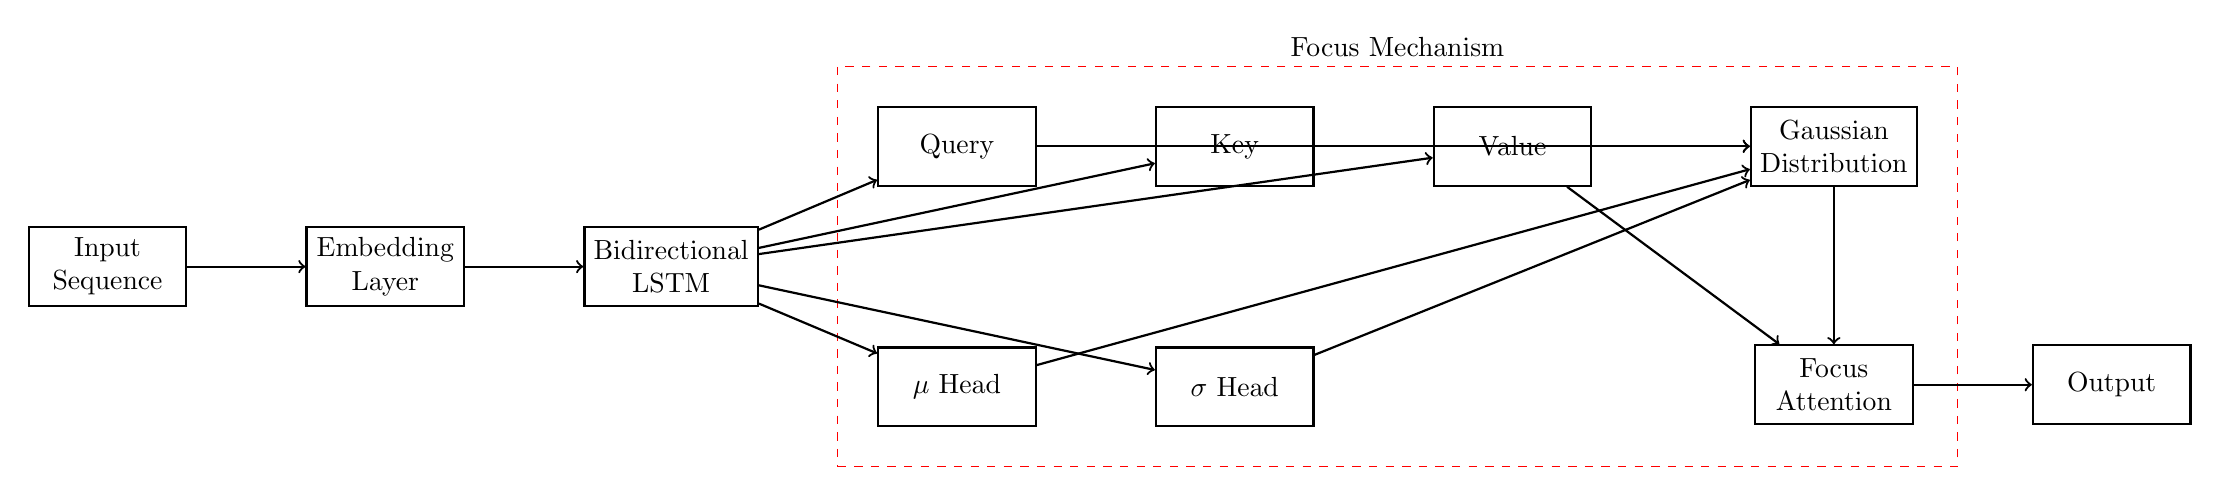
\begin{tikzpicture}[
    node distance=1.5cm,
    box/.style={rectangle,draw,minimum width=2cm,minimum height=1cm,align=center},
    arrow/.style={->,thick},
    thick
]

% Input and Embedding
\node[box] (input) {Input\\Sequence};
\node[box,right=of input] (embed) {Embedding\\Layer};

% BiLSTM
\node[box,right=of embed] (lstm) {Bidirectional\\LSTM};

% Focus Mechanism Components
\node[box,above right=0.5cm and 1.5cm of lstm] (query) {Query};
\node[box,right=of query] (key) {Key};
\node[box,right=of key] (value) {Value};

% Gaussian Parameters
\node[box,below right=0.5cm and 1.5cm of lstm] (mu) {$\mu$ Head};
\node[box,right=of mu] (sigma) {$\sigma$ Head};

% Focus Distribution
\node[box,right=2cm of value] (gaussian) {Gaussian\\Distribution};

% Output
\node[box,below=2cm of gaussian] (attention) {Focus\\Attention};
\node[box,right=of attention] (output) {Output};

% Arrows
\draw[arrow] (input) -- (embed);
\draw[arrow] (embed) -- (lstm);
\draw[arrow] (lstm) -- (query);
\draw[arrow] (lstm) -- (key);
\draw[arrow] (lstm) -- (value);
\draw[arrow] (lstm) -- (mu);
\draw[arrow] (lstm) -- (sigma);
\draw[arrow] (query) -- (gaussian);
\draw[arrow] (key) -- (gaussian);
\draw[arrow] (value) -- (attention);
\draw[arrow] (mu) -- (gaussian);
\draw[arrow] (sigma) -- (gaussian);
\draw[arrow] (gaussian) -- (attention);
\draw[arrow] (attention) -- (output);

% Background box for Focus Mechanism
\begin{scope}[on background layer]
\node[rectangle,draw=red,dashed,fit=(query)(key)(value)(mu)(sigma)(gaussian),
      inner sep=0.5cm,label=above:Focus Mechanism] {};
\end{scope}

\end{tikzpicture}
\end{document}
